\documentclass[12pt]{report}

\usepackage[utf8]{inputenc}
\usepackage[french]{babel}
\usepackage[T1]{fontenc}
\usepackage{longtable}
\usepackage{graphicx}

%-------------------------------------------------------------------------------------------------------------------------------
% Marges
\usepackage[top=2cm, bottom=2cm, left=2cm, right=2cm]{geometry}
%-------------------------------------------------------------------------------------------------------------------------------

%-------------------------------------------------------------------------------------------------------------------------------
% Entete et pied de page
\usepackage{fancyhdr} 
\fancypagestyle{plain}{%
	\fancyhf{} 
	\fancyhead{}                  
	\fancyfoot{}   
	\fancyfoot[L]{Ufwi}
	\fancyfoot[C]{\thepage}
	\fancyfoot[R]{\today}
	\chead{Projet tuteuré – Ufwi}
	\renewcommand{\headrulewidth}{1pt}   
	\renewcommand{\footrulewidth}{1pt}      
}
\pagestyle{plain}
%-------------------------------------------------------------------------------------------------------------------------------




%-------------------------------------------------------------------------------------------------------------------------------
% Gestion de l'affichage des chapitres
\makeatletter
\renewcommand{\@chapapp}{}
\makeatother
%-------------------------------------------------------------------------------------------------------------------------------

\title{Ufwi}
\author{Maxime Robin, Cyril Pierré, Valentin Frolich, Simon Barotte}
\date{\today}

\begin{document}



%-------------------------------------------------------------------------------------------------------------------------------
% Page d'accueil
\thispagestyle{empty}
\begin{center}
Licence Professionnel ASRALL


Projet tuteuré.

\vspace{2,5cm}
\textbf{\Huge Ufwi}


\end{center}


%-------------------------------------------------------------------------------------------------------------------------------

\newpage

%-------------------------------------------------------------------------------------------------------------------------------
% Sommaire
\renewcommand{\contentsname}{Sommaire}
\tableofcontents
%-------------------------------------------------------------------------------------------------------------------------------

\newpage

%-------------------------------------------------------------------------------------------------------------------------------
% Content
\chapter{Introduction}
Début du doc de Ufwi

%-------------------------------------------------------------------------------------------------------------------------------
\chapter{Liste des solutions de pare-feu par identification}
Les pare-feu par identification les plus connus : 
  \begin{itemize}
    \item AuthPF : Fonctionne sous OpenBSD et qui se repose sur SSH pour l'identification des utilisateurs : http://www.openbsd.org/faq/pf/authpf.html
    \item NuFW : projet ayant donné naissance à UFWI suite à la liquiditation de l'éditeur "EdenWall Technologies"
    \item Cyberoam : pare-feu entièrement basé sur l'identification, en utilisant une corrélation entre adresse MAC et utilisateur : http://www.cyberoam.com/fr/firewall.html
    \item CheckPoint (NAC Blade) : utilisation des règles de filtrage en fonction d'une authentifcation basée sur Kerberos, l'identité de son poste et du niveau de sécurité du poste ( mise à jour de sécurité / antivirus ) : http://www.cyberoam.com/fr/firewall.html
  \end{itemize}
%-------------------------------------------------------------------------------------------------------------------------------
\chapter{Externalisation des logs dans une BD MySQL}
\underline{Configuration du serveur BD}

Installation des paquets :

apt-get install apache2 php5 mysql-server nulog

\underline{Configuration de la passerelle : }

Configuration IP :

ifconfig eth0 192.168.1.137/24
ifconfig eth1 172.20.8.1/24

Installation des paquets :

apt-get install ulogd ulogd-mysql

Correction d'un bug : ajout d’une ligne dans le script de démarrage qui va charger un module

nano /etc/init.d/ulogd
export LD_PRELOAD=/usr/lib/libmysqlclient.so.16

Configuration de ulogd : modification de son fichier de configuration

nano /etc/ulogd.conf

Décommenter la ligne 46 (pour charger un module supplémentaire)

Renseigner les informations de connexion à la base de données :

paragraphe « [MYSQL] » ligne 59 :
table=’’ulog’’
pass=’’passulog’’
user=’’ulog’’
db=’’ulog’’
host=’’172.20.8.2’’

Configuration du serveur de BD:

Configuration IP :

ifconfig eth0 172.20.8.2/24

Lister tous les fichiers installés à l’installation de nulog :

dpkg –L nulog | more

Ouvrir le fichier suvant (démarche à suivre pour creer les tables de la base de données)

nano /usr/share/doc/nulog/README.Debian

Connexion à la base de données et création de l’utilisateur (les deux programmes vont se connecter avec ce compte):

mysql –u root –p
create database ulog;
create user 'ulog'@'\%' identified by 'passulog' ;
grant all privileges on ulog.* to ulog;
exit

Commandes de création de la base :

cd /usr/share/doc/nulog/scripts
gunzip ipv4.sql.gz
cat ipv4.sql | mysql –uulog –p ulog

Modification du fichier de configuration de mysql

nano /etc/mysql//my.cnf
ligne 47

Il faut qu’il écoute sur l’interface 172.20.8.2

bind address= ‘’172.20.8.2’’

Renommer les fichiers de configuration :

cd /etc/nulog
cp default. core.conf core.conf
cp default.nulog.conf nulog.conf
cp default.wrapper.conf wrapper.conf

Renseigner les informations de connexion à la base de données :

nano core.conf
host=localhost
db=ulog
user=ulog
password=passulog
table=ulog

Prise en compte des changements : redémarrage de services
Sur la passerelle :

/etc/init.d/ulogd restart

Sur le serveur :

/etc/init.d/ulogd restart


On choisit ce que l’on veut loguer avec iptables

%-------------------------------------------------------------------------------------------------------------------------------
\chapter{Daemon ufwi-authd}
\section{Introduction}

Nuauth command est une interface qui permet de contrôler des fonctions importantes du daemon authd, 
comme l'obtention de la liste des utilisateurs connectés par exemple.
Chaque fois qu'un client envoie un paquet(1) pour commencer une connexion à travers la 
passerelle, la station cliente envoie un paquet(2) d'identification au daemon authd. Le 
pare-feu de la passerelle met en file d'attente le paquet et envoie directement des 
informations au daemon authd.

Le travail du daemon va être d'analyser les deux paquets (1) et (2) et de vérifier si 
le client à le droit d'initialiser la connexion qu'il demande.
Si ufwi-authd indique que le paquet(1) est autorisé alors la connexion est initialisé,
sinon la connexion est annulé. Ufwi-authd peut aussi utiliser un serveur LDAP pour la
définition des utilisateurs et groupes.

Ci-dessous le un schéma montrant le processus d'authentification utilisé par NuFW, resté inchangé avec UFWI:

\begin{center}
  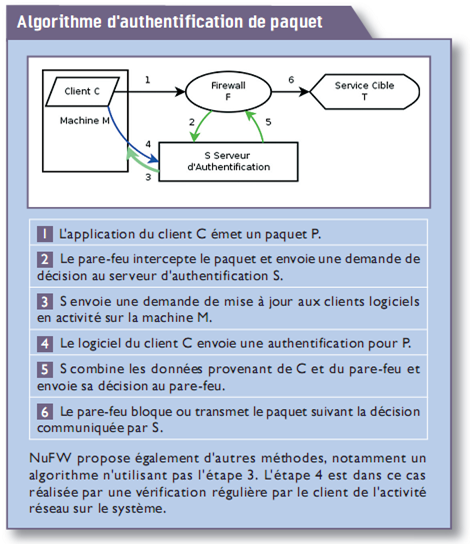
\includegraphics[width=8cm,height=10cm]{images/auth.png}
\end{center}

\section{Intallation}

Pré-requis :

Script autogen.sh :
    \begin{itemize}
      \item version automake1.7
    \end{itemize}
Compilation Nufw :
  \begin{itemize}
    \item GNU libtool
    \item GNU make
    \item libpam-dev
    \item glib 2.4+
    \item libipq (iptables-dev pour debian) ou libnetfilter queue
    \item libldap
    \item libsasl2
    \item libgnutls
    \item libgcrypt
  \end{itemize}

Noyau:

Il est recommandé d'utiliser un noyau récent afin de bénificer de toutes les dernières nouveautés implémenter dans ce dernier.
Une version de noyau supèrieur à 2.6.18 est un bon choix. Le patch dump-connection-mark.diff ( disponible dans patches/ ) 
peut être appliqué au noyau afin d'améliorer les perfomances de ce dernier lorsque nous utiliserons le log de session.

Compilation:

La compilation du daemon est relativement simple, elle se déroule en quatre étapes:
  \begin{itemize}
   \item Lancement du script ./autogen.sh
   \item Exécution de ./configure
   \item make
   \item Et pour finir make install
  \end{itemize}
Lors de la première installation, il faut penser à copier le ficheir de configuration avec la commande suivante:

cp ./conf/nuauth.conf /usr/local/etc/nuauth.conf

\section{Quelques commandes liées au daemon}

Commandes principales:
\begin{itemize}
  \item quit: déconnexion
  \item refresh cache: rafraichit tous les caches
  \item reload: recharge la configuration du daemon d'authentification 
\end{itemize}
Information:
\begin{itemize}
  \item help: affiche la liste des commandes utilisables
  \item version: affiche la version du daemon
  \item uptime: affiche depuis combien de temp tourne le daemon 
\end{itemize}
Gestion des utilisateurs:
\begin{itemize}
  \item users: affiche els utilisateurs connectés
  \item disconnect all: déconnecte tous les utilisateurs
  \item disconnect ID: déconnecte un utilisateur grâce à son identifiant (ID) 
\end{itemize}

\section{Fichier de configuration}

Le fichier authd.conf est le fichier principal de configuration pour le
daemon ufwi-authd. C'est dans ce fichier que seront indiqué l'adresse du daemon ufwi-filterd 
par exemple ou encore le niveau de debug, le nombre de connexion qu'un utilsateur peut lancer.
Dans ce fichier seront aussi renseigné les différents paramètres qui guide le comportement du 
daemon, mais aussi les paramètres système, et pour finir les chemins absolus des autres fichiers
de configuration.

Il existe aussi d'autres fichiers de configurations liés à ufwi-authd:
\begin{itemize}
  \item modules/nuauth-tls.conf qui contiendra les paramètres TLS
  \item modules/nuauth-krb5.conf configuration authentification Kerberos 5
  \item modules/nuauth-ldap.conf authentification ldap
  \item modules/nuauth-mysql.conf configuration de la base de donnée pour les logs utilisateurs (mysql)
  \item modules/nuauth-pgsql.conf configuration de la base de donnée pour les logs utilisateurs (postgres) 
\end{itemize}
 
%-------------------------------------------------------------------------------------------------------------------------------
\chapter{Daemon ufwi-filterd}
\section{Introduction}

	Le daemon ufwi-filterd (ancienement appelé nufw) n'est d'autre qu'un pare-feu basé sur NFQUEUE netfilter. Il permet d'écrire des règles de filtrage basées sur l'identité des utilisateurs, en plus des critères de réseau classiques. L'authentification effectue de façon transparente en requérant les informations d’identification de l’utilisateur avantqu’une quelconque décision de filtrage ne soit prise. En pratique, cela signifie que les politiques defiltrage peuvent intégrer l’annuaire utilisateur, et amène cette notion d’ID utilisateur au niveau de la couche IP.\\
Ufwi-filterd est capable de:
\begin{itemize}
  \item Filtrer le trafic en fonction du système d’exploitation et des applications utilisées par les utilisateurs
     distants.
  \item marquer chaque paquet d'une connexion avec l'identifiant de son utilisateur et donc d'appliquer une politique de qualité de service spécifique à chaque utilisateur. 
  \item contribue de manière très pointue à la surveillance de l'activité réseau des serveurs.
  \item dispose de modules de surveillance qui journalisent les événements principaux de l'activité du réseau en indiquant quels sont les utilisateurs à l'origine des flux.
\end{itemize}
\section{Intallation}
Une installation typique de la suite logicielle NuFW comporte 2 démons : nufw (ufwi-filterd) et nuauth (ufwi-authd) et autant de clients que nécessaire.\\
Pré-requis :
\begin{itemize}
  \item automake1.7 pour executer autogen.sh
  \item GNU libtool
  \item GNU make
\end{itemize}
Pré-requis pour la compilation et l'excution de ufwi-filterd :
\begin{itemize}
  \item ufwi-base
  \item ufwi-confparser
  \item ufwi-ssl
\end{itemize}
Il est recommandé d'utiliser un noyau récent afin de béneficer de toutes les dernières nou-
veautés implémenter dans ce dernier. Une version de noyau supèrieur à 2.6.18 est un bon choix.
\newpage
\section{Compilation}
La compilation de ufwi-filterd est relativement simple elle se resume a utiliser les commandes suivantes :
\begin{itemize}
  \item ./autogen.sh
  \item ./configure
  \item make
  \item makeinstall
\end{itemize}
Lors de la première installation, il ne faut pas oublier de copier le fichier de configuration "make install-conf" afin de chercher les changements entre votre fichier de conf actuelle et le nouveau.\\
Un fichier INSTALL avec toutes les instructions a suivre est fournie dans le dossier de ufwi-filerd disponible a partir de se lien http://ufwi.org/projects/ufwi-filterd/ repository .
\section{Commandes}
Tout dabord, vous devez executer en root ufwi-filterd.
ufwi-filterd -h vous donnera un message d'aide pour l'utilisation de ufwi-filterd.
\section{Fichier de configuration}
Le fichier de configuration de ufwi-filterd se nome tout simplement "filterd.conf". On poura le trouver dans /etc/ufwi-filterd/.
Dans se fichier on trouvera l'adresse ou le nom du serveur d'authentification nuauth (par defaut 127.0.0.1), on trouvera aussi les chemin absolut des fichiers :
\begin{itemize}
  \item /etc/ufwi-filterd/key.pem (clé privé du serveur)
  \item /etc/ufwi-filterd/cert.pem (certificat du serveur)
  \item /etc/ufwi-filterd/cacert.pem
  \item /etc/ufwi-filterd/crl.pem (liste de révocation de certificat serveur)
\end{itemize}

%-------------------------------------------------------------------------------------------------------------------------------
\chapter{Daemon ufwi-rcpd}
\section{Introduction}
Le module ufwi-rcpd (anciènnement appelé NuCentral) est le module qui gère les autres deamons.

\section{Installation}
\subsection{Pré-requis}
Avant de lancer l'installation du module, certains pré-requis sont nécéssaires :
\begin{itemize}
  \item Python 2.5
  \item Twisted web
  \item M2Crypto
  \item Jinja
  \item Subversion (svnadmin program)
  \item sudo
  \item pysvn
  \item pytz
\end{itemize}
Debian: apt-get install python-twisted-web python-svn python-m2crypto sudo python-jinja subversion python-tz
\newline

Pour l'installation de ufwi-rpcd:
\begin{itemize}
  \item (GNU) make
  \item sqlite3
\end{itemize}
Sous Debian: apt-get install make sqlite3
\newline

Paquets optionnels :
Pour compiler les fichiers de .ts à .qm et mettre à jours les transmissions :
\begin{itemize}
  \item lrelease4: Qt development tools
  \item pylupdate4, lrelease-qt4: Python Qt development tools
\end{itemize}
Sous Debian: apt-get install libqt4-dev pyqt4-dev-tools
\newline

Autres :
\begin{itemize}
  \item python-twisted-snmp : pour le module SNMP.
  \item gnutls-bin : le programme certtool l'utilise pour générer les certificats ssl.
  \item py.test (Sous Debian python-codespeak-lib) : Utiliser pour les tests.
  \item libconfig-inifiles-perl : pour tools/ufwi\_rpcd\_enmod.
  \item IPy (python-ipy) : pour les tests.
\end{itemize}


%---------------------------------------------------------------------------------------------------------------------------------
\end{document}
